\section{Xử lý và số hóa đặc trưng subject}

Đặc trưng \texttt{subject\_category} được trích xuất từ Mistral API cần được \textbf{làm sạch và chuẩn hóa} trước khi sử dụng. Quá trình xử lý này được thực hiện tại class \texttt{Processing} với các bước quan trọng:

\noindent\textbf{Làm sạch dữ liệu subject:}
\begin{itemize}
    \item \textit{Chuẩn hóa format}: Chuyển về lowercase, loại bỏ dấu ngoặc kép, dấu sao và ký tự đặc biệt
    \item \textit{Xử lý lỗi API}: Phát hiện và chuyển các response lỗi từ API (như "article snippet", "please provide", "unable to provide") về nhãn \texttt{'other'}
    \item \textit{Kiểm tra độ dài}: Các response quá dài (>6 từ) được coi là lỗi và chuyển về \texttt{'other'}
    \item \textit{Mapping về allowed categories}: Chỉ giữ lại 19 danh mục được định nghĩa trước, các giá trị khác được gán về \texttt{'other'}
\end{itemize}

\noindent Việc xử lý này cần thiết vì API có thể trả về các response không nhất quán, lỗi format, hoặc nội dung không mong muốn do prompt engineering không hoàn hảo hoặc giới hạn của model.

\noindent\textbf{Số hóa categorical data:}
Sau khi làm sạch, đặc trưng categorical \texttt{subject\_category} được chuyển đổi thành \textit{dummy variables} bằng one-hot encoding. Kết quả là 18 cột binary (bỏ 1 category làm reference) thay thế cho 1 cột categorical ban đầu.

\section{Xử lý đặc trưng text}

Cột \texttt{text} chứa nội dung bài báo cần được \textbf{tiền xử lý sâu} để loại bỏ noise và chuẩn hóa dữ liệu văn bản. Quá trình này được thực hiện qua method \texttt{clean\_text} với các bước:

\noindent\textbf{Làm sạch text:}
\begin{itemize}
    \item \textit{Loại bỏ ký tự đặc biệt}: Sử dụng regex để chỉ giữ lại chữ cái và khoảng trắng
    \item \textit{Chuẩn hóa case}: Chuyển toàn bộ về lowercase để đảm bảo consistency
    \item \textit{Stopword removal}: Loại bỏ các từ phổ biến không mang ý nghĩa phân biệt
\end{itemize}

Việc xử lý này cần thiết vì:
\begin{itemize}
    \item \textit{Giảm dimensionality}: Loại bỏ noise và các từ không quan trọng giúp giảm kích thước feature space
    \item \textit{Chuẩn hóa input}: Đảm bảo các model NLP hoạt động ổn định với input
    \item \textit{Tăng hiệu quả}: Text sạch giúp các thuật toán vectorization (TF-IDF, Word2Vec) hoạt động hiệu quả hơn
    \item \textit{Focus vào content}: Loại bỏ stopwords giúp model tập trung vào các từ mang ý nghĩa thực sự
\end{itemize}

Kết quả là cột \texttt{text} được làm sạch, chuẩn hóa và sẵn sàng cho các bước tokenization và vectorization tiếp theo.

\section{Phân tích chuyên sâu}

\begin{figure}[h!]
\centering
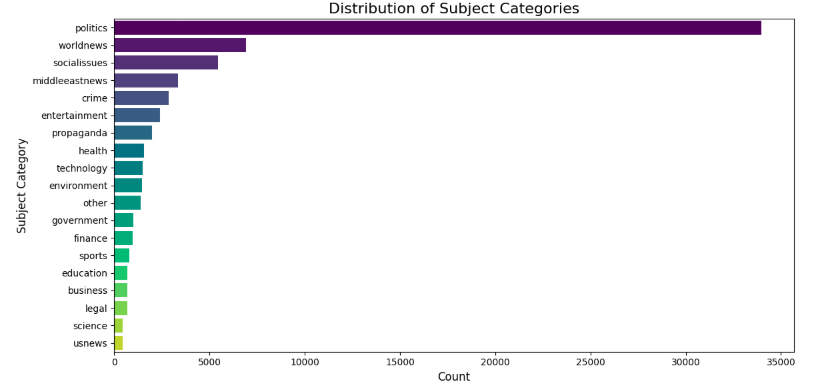
\includegraphics[width=1\textwidth]{images/3.png}
\end{figure}
\FloatBarrier
\noindent\textbf{Nhận xét:} Dataset có class imbalance nghiêm trọng với Politics chiếm áp đảo (~47\% tổng data), WorldNews đứng thứ 2 nhưng chỉ bằng 1/5. Các chủ đề còn lại rất ít, đặc biệt USNews/Science/Legal gần như không có.

\begin{figure}[h!]
\centering
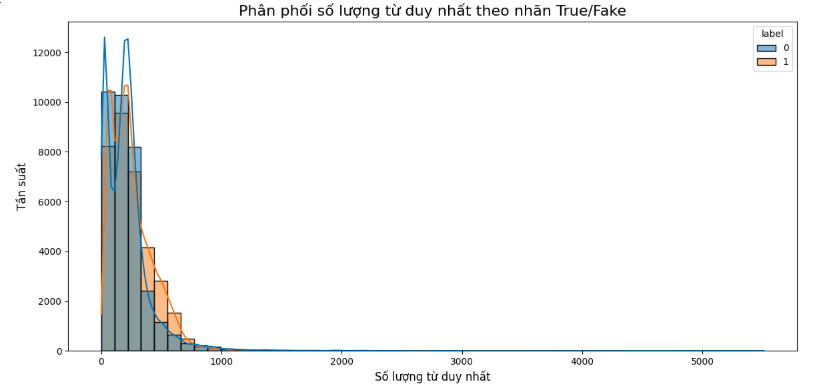
\includegraphics[width=1\textwidth]{images/4.png}
\end{figure}
\FloatBarrier

\noindent\textbf{Nhận xét:} Phân phối của cả hai nhãn đều lệch phải (skewed right), với phần lớn các bài viết có dưới 1000 từ duy nhất. Tin giả (label = 0) có xu hướng chứa nhiều từ duy nhất hơn so với tin thật (label = 1), đặc biệt rõ ở phần đuôi bên phải của phân phối. Tần suất xuất hiện của các num\_unique\_words khác nhau ở Fake news (đỉnh ở khoảng trên 12,000) cũng cao vượt trội so với True news (đỉnh ở khoảng trên 10,000)

\begin{figure}[h!]
\centering
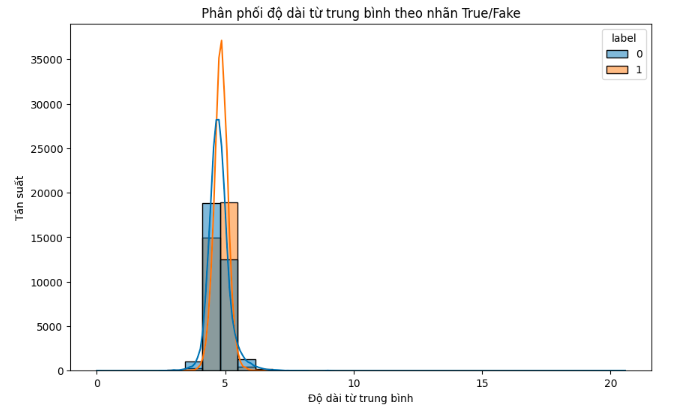
\includegraphics[width=1\textwidth]{images/5.png}
\end{figure}
\FloatBarrier

\noindent \textbf{Nhận xét:}
\begin{itemize}
    \item Tin thật (label = 1) có phân phối hẹp hơn và đỉnh cao hơn, cho thấy các bài viết thật sử dụng từ với độ dài trung bình ổn định và ít biến động hơn.
    \item Tin giả thường dùng từ ngắn hoặc dài không đồng đều → có thể là dấu hiệu của việc sử dụng từ ngữ gây sốc, giật gân hoặc không tự nhiên.
\end{itemize}
\begin{figure}[htbp]
    \centering
    \begin{minipage}{0.48\textwidth}
        \centering
        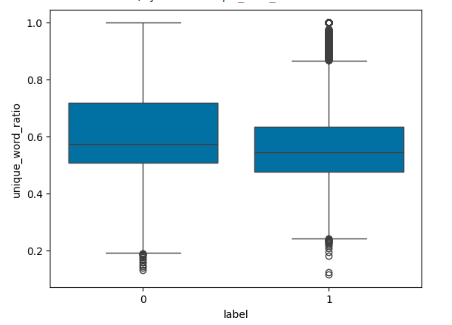
\includegraphics[width=\textwidth]{images/6.png}
        \label{fig:hinh1}
    \end{minipage}
    \hfill
    \begin{minipage}{0.48\textwidth}
        \centering
        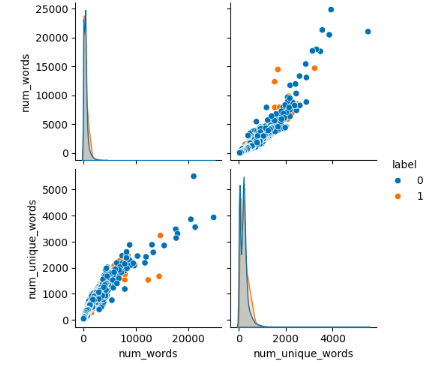
\includegraphics[width=\textwidth]{images/7.png}
        \label{fig:hinh2}
    \end{minipage}
\end{figure}
\noindent \textbf{Nhận xét:} Trung vị (median) của unique\_word\_ratio ở tin thật (1) thấp hơn so với tin giả (0). Tin giả (0) có phạm vi dao động (IQR) và cả phân bố trên (upper whisker) cao hơn → nhiều bài viết giả có tỷ lệ dùng từ duy nhất cao. Tin giả thường có tỷ lệ từ duy nhất cao hơn, cho thấy chúng có thể được viết theo cách cố tình đa dạng từ vựng hoặc khó đoán hơn, trong khi tin thật thường dùng từ ngữ nhất quán hơn. Chú ý vào 2 biểu đồ scatter , ta nhận thấy có mối quan hệ tuyến tính khá rõ giữa số lượng từ và số lượng từ duy nhất trên cả 2 label.

